\chapter{Designing the linking function}\label{Chap:ML}
As discussed in previous Chapter \ref{Chap:LLFs}, we formalize the signal domain by means of a feature-based representation. The representation based on hand-crafted and model-based features only provides little insight on the semantics of the music, while the representation based on deep learning architecture requires manual inspection in order to assess its semantics \cite{Le2013,choi2015auralisation}. The semantic domain, which we will  better discuss in the next Chapter \ref{Chap:HLFs}, provides a high-level description of music, that is closer to the way people describe and think of music. The relation between the signal domain, related to the lower-level properties of the musical content, and the semantic domain, related to the high-level interpretation of music, is often not clear, due to the well-known semantic gap between low-level and high-level features \cite{Celma2006}. In this Section, we discuss several techniques that have been employed in the literature to bridge the gap in the Music Information Retrieval research field. 

The design of the linking function involves different techniques, depending on the complexity of the addressed problem and on the available knowledge on the relation between the domains for the specific problem. For some cases, when it is possible to make some assumption on the relation between the two domains, rule-based techniques can be designed and employed. More often, however, the problem that is addressed involves the understanding of the human music's perception, whose modeling is extremely complex and still under investigation. For the latter cases, we take advantage of machine learning techniques to design and train the models for linking function. 

In the following, we provide an overview of the theoretical background and the state of the art of some techniques used in the literature to model the linking function. In Section \ref{sec:ML:data} we first present some basic tools to pre-process the representation of the signal or the semantic domain to help de-noising the data, to improve the effectiveness of the linking function. In Section \ref{sec:ML:kernels} we describe a set of kernel expansion techniques that we used in our work to expand the data and explore possibly underlying patterns within it. In Section \ref{sec:ML:rule-based} we present a set of tools to design rule-based techniques. We focus on the techniques that have been used in the literature to automatically extract the musical structure of songs, since this is a common problem in Music Information Retrieval. Finally, in Section \ref{sec:ML:models} we present a number of machine learning techniques that have been proposed to automatically learn a model for the linking function.

%The design of automatic music mediators can be modeled as a function that links the representation of the signal domain (Chapter ) to the formalization of the semantic codomain (Chapter \ref{Chap:HLFs}). Therefore, the properties of the linking function strongly depend on the two domains. The novel mediator can also be seen as a pipeline that connects the the signal domain to the linking function, and the linking function to the the semantic codomain. From this perspective, the source needs to be adapted to the blocks afterwards, i.e., the formalization of the signal domain must be shaped for the linking function, which must be accurately chosen to address the semantic codomain.

%The linking function handles the representation of the signal domain, which might need to be shaped and modified in several ways. Firstly, a regularization is often necessary in order to make the extracted features uniform with respect to their range. Then, we must define a metric distance between the samples in the signal domain. For this purpose, linear metrics such as the Euclidean distance are commonly employed, but they might be insufficiently descriptive. We can increase the level of descriptiveness by introducing some nonlinearity in the input space of the music representation, to explore further relationship among features, and the distance among samples can be learned with machine learning techniques in order to match some external requirements. Finally, for some analysis the representation of the interaction among samples can be more informative than the representation of the samples themselves. We can compute a \textit{self-similarity} or \textit{self-distance} matrix to provide this information.

%After the signal domain has been shaped, the linking function must be chosen in order to be able to represent the desired semantics of the codomain. As we discussed in Section \ref{sec:HLFs:anns}, the scenario of annotating music with a categorical approach can be seen as a case of classification of music into different non-overlapping categories. In this case, the best approach is to use classifiers, i.e., machine learning techniques for the prediction of discrete values. When a dimensional model has been chosen to formalize the semantic codomain, instead, the  linking function needs to return values in a continuous range. Machine learning techniques called \textit{regressors} can be used for this scenario. Finally, when analyzing a problem where the semantic codomain is well formalized, such as the music structure, rule-based techniques can be employed.

%In this Chapter we present the techniques we employ in our work to model the linking function between the two domains. 
%In Section \ref{sec:ML:data} we analyze the techniques to: regularize the feature representation from signal domain; include nonlinearity; learn a distance metric in the input space; build a representation of the inner structure of the songs. 
%In Section \ref{sec:ML:models} we discuss a set of machine learning and rule-based techniques to infer the linking function for different formalizations of the semantic codomain.


%As an example, the features extracted for the representation have often different range of values, as seen in Section \ref{sec:LLFs:hand-crafted}. The linking function does not have the apriori knowledge of the range of each feature, therefore it is hard to model a technique that can handle such variety. For this reason, some kind of regularization is usually applied. 
%Some other algorithms exploit nonlinear properties of the data using a kernel to expand it in a nonlinear dimensional space. 

\section{Pre-processing techniques}\label{sec:ML:data}  
Dealing with feature-based representations of the musical content, it is frequent that the extracted features assume different ranges of values, depending on the property they capture. As an example from Section \ref{sec:LLFs:hand-crafted}, Spectral Centroid $SC$ defines a frequency, hence it ranges from 0 to half of the sampling rate, while the tempo defines an amount of beats per minute, hence it typically ranges from $20$ to $240$ BPM. 

For this reason, it is common practice to analyze and pre-process the data, before applying the rule-based or machine learning techniques. Such pre-processing techniques aim to make the range of representation uniform, and to possibly de-noise the representation. 

As a matter of fact, machine learning techniques have been proven to dramatically improve their performance when the input data is pre-processed by means of \textit{regularization} techniques \cite{PAMI}. The two main approaches to do it are normalization and standardization. 

We consider a set of $N$ items  $\mathcal{X}=\{\mathbf{x}_1,...,\mathbf{x}_N\}$, where each item $\mathbf{x}_i \in \mathbb{R}^{M}$ is a vector representation composed of $M$ components (e.g., features for the signal domain or descriptors for the semantic domain).  We refer to the representation for the entire dataset as $\mathbf{X}\in \mathbb{R}^{N \times M}$, as composed by the stacking of the vector representations, therefore the generic row of the matrix $\mathbf{X}$ is the vector  $\mathbf{x}_i$, while we refer to the generic column as $\mathbf{X}^{(m)}\in \mathbb{R}^{N \times 1}$ with $m=1,...,M$. Finally, a specific component is identified as $\mathbf{x}_{i}^{(m)}\in \mathbb{R}$.

The normalization aims to reduce the ranges for each feature to the range $[0,1]$, which can be easily achieved by defining:
\begin{equation}
x_{\text{min}}^{(m)}=\min(\mathbf{X}^{(m)}) \quad \forall m=1,...,M;
\label{eq:ML:normMin}
\end{equation}
\begin{equation}
x_{\text{max}}^{(m)}=\max(\mathbf{X}^{(m)}) \quad \forall m=1,...,M;
\label{eq:ML:normMax}
\end{equation}
and computing the normalized dataset $\tilde{\mathbf{X}}\in \mathbb{R}^{N \times M}$ as
\begin{equation}
\tilde{\mathbf{X}}=\left[ \frac{x^{(m)}_{i}-x_{\text{min}}^{(m)}}{x_{\text{max}}^{(m)}-x_{\text{min}}^{(m)}} \right] \quad \forall i =1,..., N \quad \forall m = 1,..., M
\end{equation}

The standardization aims at shaping the distribution of the values as a normal distribution with zero mean and unitary standard deviation, i.e., given
\begin{equation}
\mu^{(m)}=\frac{\sum_{i=1}^{N}\mathbf{x}_i^{(m)}}{N} \quad \forall m=1,...,M, 
\label{eq:ML:standMean}
\end{equation}
\begin{equation}
\sigma^{(m)}=\sqrt{\frac{\sum_{i=1}^{N}\left(\mathbf{x}_i^{(m)} - \mu^{(m)} \right)^2 }{N} }\quad \forall m=1,...,M;
\label{eq:ML:standStd}
\end{equation}
we compute the standardized dataset $\tilde{\mathbf{X}}$ as 
\begin{equation}
\tilde{\mathbf{X}}=\left[ \frac{x^{(m)}_{i}-\mu^{(m)}}{\sigma^{(m)}} \right] \quad \forall i =1,..., N \quad \forall m = 1,..., M.
\end{equation}

When using supervised machine learning techniques, it is common to split the dataset $\mathcal{X}$ in (at least) two subsets: the \textit{training set} $\mathcal{X}_{\text{train}}$ and the \textit{test set} $\mathcal{X}_{\text{test}}$. The former is used in the training stage to learn the parameters of the model, while the latter is used to estimate the performance of the learned model by evaluating its predictive power. In order to reliably evaluate the model, the training set must not leverage any information from the test set. For this reason, the regularization is performed by computing the parameters of Equations \ref{eq:ML:normMin}, \ref{eq:ML:normMax}, \ref{eq:ML:standMean}, \ref{eq:ML:standStd}, over the songs of the training set $x_i \in \mathcal{X}_{\text{train}}$. The parameters are used to regularize both the training $\tilde{\mathbf{X}}_{\text{train}}$ and test set  $\tilde{\mathbf{X}}_{\text{test}}$.
%\dfrac{num}{den}


\section{Expanding information by using kernel techniques}\label{sec:ML:kernels}
The linking function, either modeled with rule-based or machine learning techniques, aim to define the relation between the representations of the domain and the codomain of the addressed problem. The relation between the two domains commonly depends on some patterns of the input representation, which are detected by exploring the relation among the input samples or even among the components within each sample. Many linking function techniques are designed to use linear metrics in the space of the input representation. Such linear metrics are easy to use and often computationally cheap, but they rely on the assumptions that the components are independent with respect to each other and that the relation among samples is linear with respect to their components. In this Section we review the techniques that aim at overcoming such assumptions by considering nonlinear metrics.

%In order to do so, the linking function explores the relation between the components of the input representation and the chosen target. For some scenarios, the interaction among the samples in the domain, or even among the components within the samples, is helpful to detect patterns that are related to the codomain of the problem. While some linking function techniques can explicitly explore such interactions, some others might be designed in a more generic way, and miss useful information from the representation of the domain. As an example, the common approach to explore the interaction among samples relies on linear metrics, such as the Euclidean or Cosine distance, since they are easy to use and computationally cheap. Such metrics implicitly assume that the components are independent among each others and the similarity between samples is linear with respect to their components. We might like to overcome such assumptions.

There are two main approaches to include the nonlinearity in the metric space of the input representation. The first approach defines an explicit mapping function $\phi$ from the linear input space to a new space that is nonlinear with respect to the inputs. A linear distance computed over the nonlinear space can be interpreted as a nonlinear distance over the original space. This approach allows the use of the defined linear distances, but the dimensionality of the new space is often too high, which increases the computational cost. The second approach addresses the dimensionality issue by defining an implicit nonlinear metric $k$ in the input space. Since the implicit metric, called \textit{kernel}, is often a cheaper solution, the explicit approach is referred to as \textit{kernel trick} \cite{Smola2004}. 

In our work, we employ two of the most commonly used kernels: the polynomial kernel and the Radial Basis Function (RBF) kernel. The former aims at including the relation among features with different degrees of polynomial expansion; the latter models the distance between two samples as an exponential decay. 

The polynomial kernel aims at retrieving a metric of distance 
\begin{equation}
k(\mathbf{x}_i,\mathbf{x}_j)=||(\mathbf{x}_i-\mathbf{x}_j)||^d,
\end{equation} 
with $\mathbf{x}_i$ and $\mathbf{x}_j$ two generic frames. The same result is achieved by computing the Euclidean distance of the polynomial expansion of the samples \cite{Smola2004}. As an example, the polynomial expansion of the frame $\mathbf{x}_i$ with degree $d=2$ is 
\begin{equation}
\begin{split}
\phi(\mathbf{x}_i) = [& 1, \mathbf{x}_i^{(1)},...,\mathbf{x}_i^{(M)}, \\
 & \left(\mathbf{x}_i^{(1)}\right)^2, ...,  \left(\mathbf{x}_i^{(M)}\right)^2, \\
 & \mathbf{x}_i^{(1)} \mathbf{x}_i^{(2)}, ..., \mathbf{x}_i^{(1)} \mathbf{x}_i^{(M)}, ..., \mathbf{x}_i^{(M-1)} \mathbf{x}_i^{(M)}]. 
\end{split}
\end{equation}

On the one side, the higher the degree of the polynomial, the higher the degree of freedom and flexibility of the expanded representation and of the accuracy of the kernel. On the other side, the excessive number of components might lead to overfit the linking function to some particular region of the feature space. For this reason, in our work we only use polynomial kernels with degree 2 and 3. We highlight that using the polynomial kernel allows the linking function to exploit not only the information of the single components, but also the relations of each component with all the others.

The Radial Basis Function (RBF) kernel \cite{Smola2004} is defined as the exponential distance 
\begin{equation}
k(\mathbf{x}_i,\mathbf{x}_j)=\exp(-\gamma||\mathbf{x}_i-\mathbf{x}_j||^2),
\end{equation}
where $\gamma$ is a scalar parameter that controls the exponential decay. When using a linear system that makes use of the Euclidean distance, however, it is necessary to find an explicit kernel expansion for the RBF. In \cite{rahimi2009weighted}  the authors propose an approximation of the expansion by randomly sampling the Fourier transformation of the kernel. The result is a function $z(\mathbf{x})$ such that 
\begin{equation}
z(\mathbf{x}_i)-z(\mathbf{x}_j)\simeq \phi(\mathbf{x}_i)-\phi(\mathbf{x}_j) = k(\mathbf{x}_i,\mathbf{x}_j),
\end{equation}
where $\phi$ is the theoretical exact mapping induced by $k$.

\section{Background of rule-based techniques}\label{sec:ML:rule-based}
The relation between the signal and semantic domain often involves the way people physiologically and psychologically perceives music. The process of perception is still mainly obscure and hard to be modeled. For some scenarios, however, the relation between the signal domain and the semantic domain is sufficiently known and easy to model, and it is possible to design the linking function by means of rule-based techniques. The rule-based techniques are task-oriented, therefore a comprehensive discussion of them would be beyond the scope of our work. In this Section, we present the techniques that have been used in our thesis, which are related to the task of the automatic analysis of music structure. In order to do so, we will first provide a brief introduction about an intermediate data structure which is commonly employed for the music structural analysis (MSA), i.e., the self-similarity (or self-distance) matrix.

\begin{figure}[tb]
        \centering
      \subfloat[Self-Similarity Matrix computed from the MFCC representation of \textit{Down with the Sickness}]{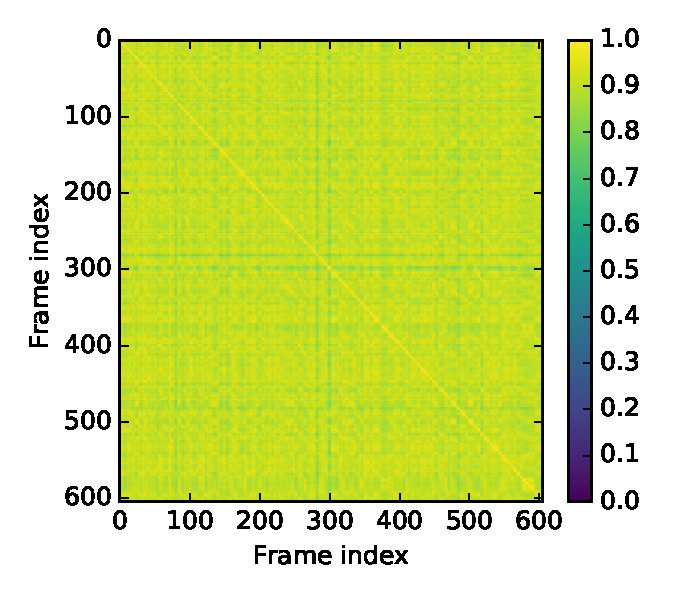
\includegraphics[width=.48\textwidth]{img/ML/mfcc_Down}\label{fig:ML:SSM_mfcc_Down}} \hfil
      \subfloat[Self-Similarity Matrix computed from the MFCC representation of \textit{Orinoco Flow}]{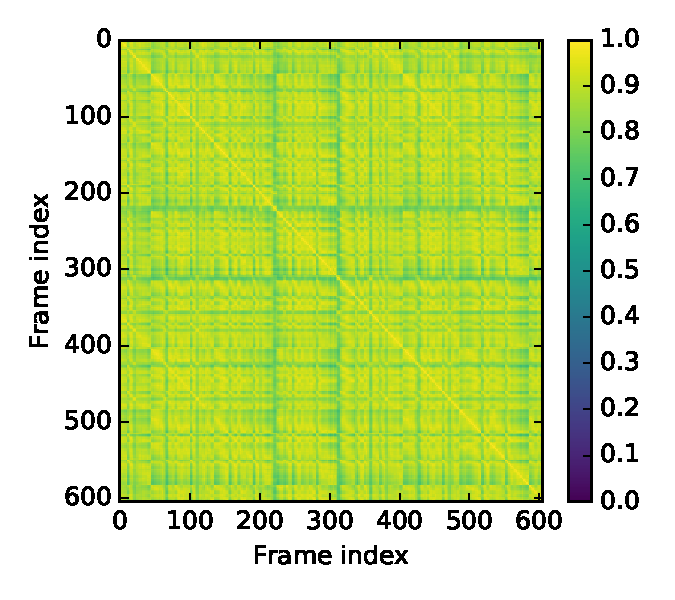
\includegraphics[width=.48\textwidth]{img/ML/mfcc_Henya}\label{fig:ML:SSM_mfcc_Henya}}
        \caption{Examples of Self-Similarity Matrices from MFCC representation}
        \label{fig:ML:SSMs_mfcc}         
\end{figure}

\subsection{Self-Similarity and Self-Distance Matrices}\label{sec:ML:self}
During the design of the linking function, it is often useful to compute the distance among pairs of samples from the input data. %In the case of the signal domain, we usually compute the distance between the representation of different songs, to estimate the similarity between them. 
Several approaches for MSA requires to estimate the inner-song similarity by computing the distance among pairs of frames' representation within the same sample, i.e., the \textit{self-similarity} matrix (SSM).

Given a song representation $\mathbf{S}$ composed of $F$ frame representations $\mathbf{s}_1,..., \mathbf{s}_F$ and a generic distance function $d: \mathbb{R}^{M} \times \mathbb{R}^{M} \rightarrowtail \mathbb{R}$, a \textit{self-distance} matrix is computed as:
\begin{equation}
\mathbf{D}=[d(\mathbf{s}_{i}, \mathbf{s}_{j})] \quad \forall i,j= 1,...,F,
\end{equation}
with $\mathbf{D} \in \mathbb{R}^{F \times F}$. 

The self-similarity matrix is the opposite of the self-distance matrix and it is computed as 
\begin{equation}
\mathbf{M}=1-\tilde{\mathbf{D}},
\end{equation}
where $\tilde{\mathbf{D}}$ is the normalized self-distance matrix. 

The self-similarity and the normalized self-distance matrix carry the same information: the former assigns higher values to closer samples, while the latter assigns higher values to the samples that are far apart. For this reason, sometimes the self-distance matrix is used as a representation of the (inverse) self-similarity.

Depending on the song, on the extracted feature and on the distance function that are used, the SSMs can remarkably vary, hence we can infer different insight on the inner organization of the songs. In Figures \ref{fig:ML:SSMs_mfcc} and \ref{fig:ML:SSMs_chroma}  we show a set of SSMs for the two songs \textit{Orinoco Flow} by the artist Henya and \textit{Down with the Sickness} by the band Disturbed, computed starting from their MFCC (Fig. \ref{fig:ML:SSMs_mfcc}) and chromagram (Fig. \ref{fig:ML:SSMs_chroma}) representations. We see that the matrices generated from the timbral features MFCCs (Figs  \ref{fig:ML:SSM_mfcc_Down} and  \ref{fig:ML:SSM_mfcc_Henya}) exhibit a rather high self-similarity (above $0.7$s) throughout the entire song. Since the timbre is linked to the sound quality of the instruments, we infer that the songs hold the same set of instruments throughout the song, even if some little change of the sound can be seen in \textit{Orinoco Flow} around frames 200 and 300. By visually inspecting the matrices computed from the chromagram representation (Figs  \ref{fig:ML:SSM_chroma_Down} and  \ref{fig:ML:SSM_chroma_Henya}), it is clear that \textit{Orinoco Flow} presents two main musical patterns, which result in a checkerboard-like matrix, while \textit{Down with the Sickness} is more harmonically uniform.

      

\begin{figure}[tb]
        \centering      
 	  \subfloat[Self-Similarity Matrix computed from the chromagram representation of \textit{Down with the Sickness}]{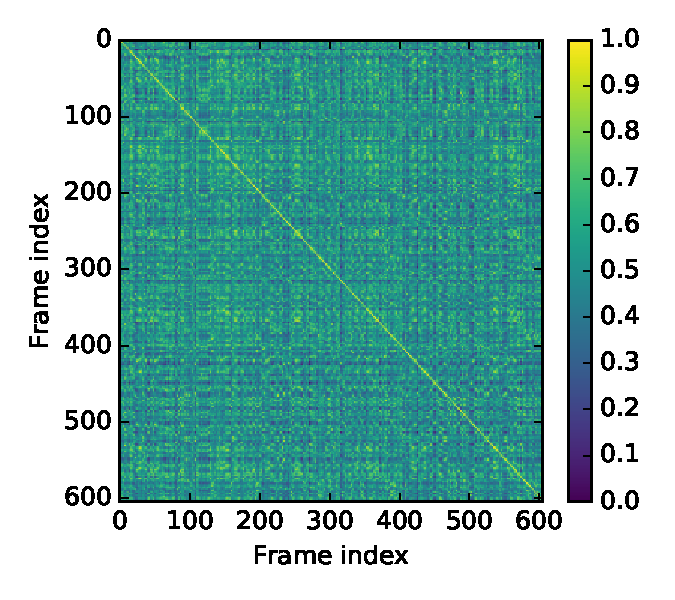
\includegraphics[width=.48\textwidth]{img/ML/chroma_Down}\label{fig:ML:SSM_chroma_Down}} \hfil
      \subfloat[Self-Similarity Matrix computed from the chromagram representation of \textit{Orinoco Flow}]{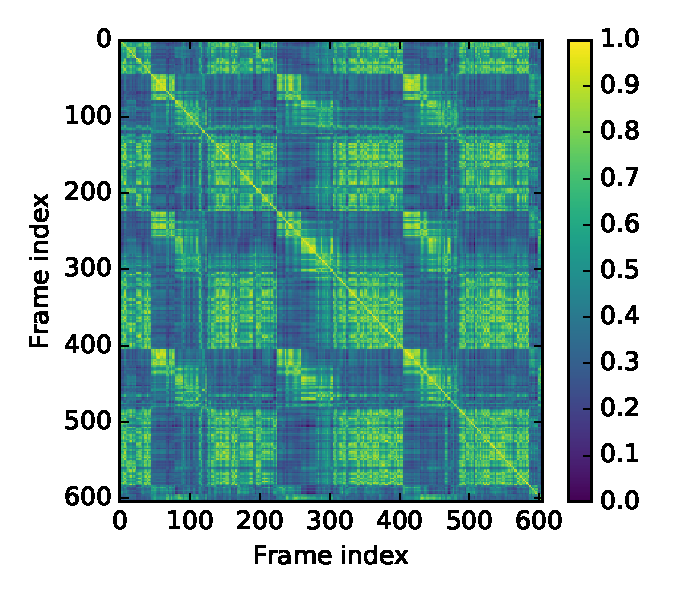
\includegraphics[width=.48\textwidth]{img/ML/chroma_Henya}\label{fig:ML:SSM_chroma_Henya}}
      \caption{Examples of Self Similarity Matrices computed from chromagram representation}
      \label{fig:ML:SSMs_chroma}         
\end{figure}

%While the SSMs are especially used in the context of MSA, the information they provide can be useful for a number of other tasks. In Chapter \ref{Chap:HLFs}, for example, we will compute the SSMs for the data drawn from a dataset for the semantic domain, in order to infer semantic similarity among descriptors.


\subsection{Music Structure Analysis techniques}\label{sec:ML:MSA}
For the Music Structure Analysis (MSA), it is known that the relation between the signal and semantic domains involves the homogeneity of some properties of the musical content or the repetition of musical patterns. This has allowed the MIR community to develop several rule-based techniques to automatically extract the music structure of a song. In this Section we provide an overview of the techniques we use in Chapter \ref{Chap:MSA}.% to address a problem in the context of MSA. Most techniques use a self-similarity or self-distance representation of the songs as presented in previous Section \ref{sec:ML:self}.

The MSA concerns the segmentation of a song into semantically meaningful segments named \textit{sections}, that represents the high-level structural composition of a song, such as \textit{verses}, \textit{chords}, \textit{bridges}, and so on. The MSA involves a first step where the boundaries between sections are detected, and a second step where retrieved sections are grouped together with regard to their role into the song. A more comprehensive discussion on the semantics of the music structure is provided in Chapter \ref{Chap:HLFs}.

One of the first and most popular MSA techniques was proposed by \cite{foote2000automatic}. The basic idea is to extract a curve from the self-similarity matrix that indicates where some novel content appears, and find the peaks of such \textit{novelty curve} to detect the boundaries among sections of the structure. More specifically, the novelty curve is computed by applying a checkerboard filter over the diagonal of the self similarity matrix. The application of the checkerboard filter spots the difference between two consecutive blocks of the self-similarity matrix. It is possible to tune the size of the kernel in order to have a smoother or sharper novelty function and hence be able to detect the boundaries at different time scales, i.e., at different hierarchical levels. 

In \cite{NietoCNMF}, a method based on the factorization of the self-similarity matrix  is proposed. Specifically, it employs a Convex Non-Negative Matrix Factorization (C-NMF) that has some useful properties. The non-negative constraint makes the factorization able to extract a representation of the self-similarity matrix as a sum of components, where the components are called the \textit{basis} of the matrix and the sum is defined by the \textit{activations}. The C-NMF adds the convexity constraint on the basis of the factorization, which must be drawn from the self-similarity itself. Consequently, the C-NMF technique factorizes the self-similarity matrix into a set of components, that represent the sections of the song's structure.

The self-similarity matrix contains the information on the similarity between frames within a song. This information can also be modeled as a graph, where the nodes are represented by the frames of the songs and the edges between nodes are represented by the similarity or the distance between the frames. 

The technique developed by \cite{jensen2005causal} exploits the graph representation to detect the boundaries between sections as the minimum path of the graph from the first to the last frame. The value of the edge between the $i$-th and the $j$-th frame is computed as the sum of the components in the sub-matrix between the $i$-th and the $j$-th rows and columns of the self-distance matrix. The values of the edges are then regularized by the time-distance of the frame (i.e., $j-i+1$) and an offset $\alpha$ is added to model the cost of creating a new segment. The nodes in the shortest path of the obtained graph detect the boundaries between sections. The parameter $\alpha$ defines how much is convenient to create a new segment, so tuning $\alpha$ help to obtain a segmentation at different levels.

The graph representation is also used by \cite{mcfee2014} to apply spectral clustering techniques, which aim at partitioning a graph into different subgraphs by cutting the low-value edges.
As in \cite{jensen2005causal}, this algorithm processes a graph representation of the self-similarity matrix in order to apply graph techniques and find a partition that reflects the musical structure of the song. In particular, the graph is computed from a binary recurrence matrix, i.e., a matrix $ \mathbf{R} \in \{0,1\}^{F \times F}$, where each element $ \mathbf{R}(i,j)$ is equal to 1 if the feature representation of the $i$-th and $j$-th frame are mutually nearest neighbors and to 0 otherwise. This approach leads to detect the boundaries of two different sections as the split of the graph between consecutive frames with a higher distance.

Finally, the algorithm proposed in \cite{Serra2014} uses a different representation of the input, by defining a set of so-called \textit{structure features} (SF) to perform the boundary detection. The structure features are built by wrapping different samples in the same row, i.e., the $f$-th row of the SF matrix representation is made by considering the previous and next frames with respect to the $f$-th frame. This helps in incorporating some time-information in the structure, making it more robust to short-time variations. The SF matrix is then smoothed with a Gaussian Kernel and a novelty function is computed between consecutive rows. The boundaries between sections are detected as peaks in the novelty curve as made by \cite{foote2000automatic}.

%In Chapter \ref{Chap:MSA} we will present a research study of ours that makes use of the abovementioned techniques to address an application scenario of MSA.

\section{Machine Learning Techniques}\label{sec:ML:models}
Machine learning techniques have been effectively used in MIR literature to model the human perception of the music. The machine learning models involves the retrieving of patterns in the input data (unsupervised models) or the prediction of an outcome from the representation of the input (supervised models). In this section we present an overview of the machine learning techniques used as a linking function for a number of scenarios.

In Section \ref{sec:ML:clust} we first present a set of clustering techniques, which aims at retrieving some patterns in the input data by grouping together samples that share some properties. Commonly, the algorithms for clustering are used as an unsupervised approach, so they do not have any clue on the patterns they are expected to retrieve. In some cases, however, the clustering techniques are adapted to embody some prior knowledge as constraints (semi-supervised techniques). The clustering techniques rely on a metric of distance between samples, which is commonly a linear metric such as the Euclidean distance. In some cases, however, it might be helpful to use a different metric that makes some pattern between samples explicit. In Section \ref{sec:ML:dist} we present the distance learning techniques, that aim at defining a metric of distance from a set of prior constraints on the data. Finally, in Sections \ref{sec:ML:classifiers} and \ref{sec:ML:semantics} we present a set of supervised machine learning techniques for the prediction of a categorical or dimensional outcome, respectively. The supervised techniques are able to learn a predictive model from a set of labeled data. It is worth remembering that, as discussed in \ref{sec:ML:data}, for supervised techniques it is common to train the model with a subset of the data (the training set) and evaluate the model with the rest of the data (the test set). Such evaluation is referred to as test error, while the evaluation computed over the training set is referred to as training error. 

In this section we follow the formalization introduced in Section \ref{sec:ML:data} for the design of the linking function. Given the dataset $\mathcal{X}=\{x_1,...,x_N\}$, we refer to the relative counterpart in the codomain of the problem as the dataset $\mathcal{Y}=\{y_1,...,y_N\}$ and to the whole possibly annotated dataset as $\mathcal{D}=\{(x_1, y_1),...,(x_N, y_N)\}$. The generic codomain image $y_i$ receive several formalizations depending on the addressed problem and the designed linking function. %we are not using the bold font because the outcome might not be a vector. 
%In the following Sections we will present the formalization of the codomain for the specific use cases.


\subsection{Unsupervised and Semi-Supervised Clustering}\label{sec:ML:clust}
A clustering method is a usually unsupervised technique that aims at grouping a dataset of samples based on a given definition of distance or similarity \cite{PAMI}. Several techniques have been proposed in the literature, aiming at grouping samples with different shapes or by exploiting various principles \cite{jain1999data}. Since a comprehensive discussion is beyond the scope of our work, we present here the approaches we use for our work.

The K-Means \cite{macqueen1967some} algorithm is one of the most widely used unsupervised clustering technique. Given an initial set of $K$ candidates for centroids, the algorithm involves two steps that are iterated until convergence: 
\begin{enumerate}
	\item each sample is assigned to the closest centroid, i.e., to the correspondent cluster;
	\item the position of the centroids are updated in order to represent the actual centroids of the samples in their cluster.
\end{enumerate}
The K-Means algorithm requires the user to select the desired number of clusters $K$, which is often not known in advance.  Moreover, the choice of the initial set of centroids is crucial in the resulting clusters, so it needs to be accurate. 

The X-Means algorithm is proposed by \cite{Pelleg2000} to overcome the former limitation. The algorithm runs the K-means algorithm several times, for each $K=K_{min},...,K_{max}$, and chooses the $K$ and clustering that exhibits the higher quality measure. The authors propose two measures: the Bayesian Information Criterion (BIC) and the Akaike Information Criterion (AIC) measures.

The latter limitation is usually addressed by choosing a random set of samples as the initial candidates for the centroids, and running the K-means algorithm for a number of times, each time with a different random set of candidates, in order to choose the set that best describes the data for some objective metrics \cite{PAMI}. An algorithm for the selection of the initial set of candidates is also proposed in \cite{Arthur2007}.

The K-means algorithm is especially effective in retrieving clusters with a globular shape \cite{PAMI} (i.e., with similar variance in all the dimensions), since each cluster aggregates the data around a centroid. In order to retrieve clusters with a different shape, other techniques might be more effective. 

The Agglomerative Hierarchical Clustering \cite{sibson1973slink} (AHC) follows a hierarchical bottom-up approach to build the clusters. At first, each sample is assigned to a different clusters, so we have $M=N$ clusters. Iteratively, the two closest clusters in the set merge together, leading to $M-1$ total clusters. The clusters keep merging until the desired final number of clusters $K$ is reached. %The algorithm can lead to different 
The final clustering results depend on which metric is used to estimate the distance between two clusters. The most common metrics are \cite{Tan2005}:
\begin{itemize}
	\item the \textit{complete-linkage clustering}, which considers the maximum distance between the samples in the two clusters; 
	\item the \textit{single-linkage clustering}, which considers the minimum distance between the samples in the two clusters; 
	\item the \textit{average-linkage clustering}, which considers the average distance between the samples in the two clusters; 
	\item the \textit{centroid-linkage clustering}, which considers the distance between the centroids of the two clusters.
\end{itemize}

In Section \ref{sec:ML:MSA} we reviewed the Spectral Clustering and Non-Negative Matrix Factorization (NMF) for the MSA task. The two approaches have originally been employed for clustering of data. 

The Spectral Clustering \cite{shi2000normalized} (SC) technique processes a graph built from the input data, with the nodes given by the samples and the edges defined by the distances between them. The SC technique looks for the lowest cost partition of the graph, by evaluating  the \textit{normalized cut}, which is a measure of the dissociation between two cluster that considers both the weights of the edges between the two groups and the weights of the edges of each group with respect to the overall graph. This approach ensures that the final cut is made between well separated and well balanced clusters. The basic SC algorithm cuts a graph, i.e., a dataset, into two groups, and can be used recursively to obtain $K$ clusters. In \cite{shi2000normalized} the authors propose an approach to generalize the algorithm to cut the graph into $K$ subgroups.

In \cite{xu2003document} the authors propose an algorithm for clustering based on a Non-Negative Matrix Factorization. The NMF is used to decompose a matrix into a positive sum of the main components, which, in this case, represent the main clusters. More specifically, this approach processes the input data representation $\mathbf{X}$ in order to compute two matrices $\mathbf{U}$ and $\mathbf{V}$ representing the cluster centroids and the clusters' association respectively.

The clustering of samples is a commonly unsupervised task. However, some algorithms are adapted to be trained in a semi-supervised fashion, in order to consider some desiderata on the final clustering, by providing a set of constraints. Two sets of constraints are defined, the Must-Link $ML$ and Cannot-Link $CL$, that collect the samples that must be or must be not grouped together, respectively.

In \cite{chen2008} the authors propose a Semi-Supervised approach for the algorithm based on Non-Negative Matrix Factorization (SS-NMF). This approach uses the distance matrix $\mathbf{D}$ computed from the sample of the input data $\mathbf{X}$ instead of the data itself. The distance matrix is processed in order to include the information from the $ML$ and $CL$ sets as  
\begin{equation}
\hat{\mathbf{D}}=[\mathbf{D}(i,j) - \zeta_{i,j} + \vartheta_{i,j}] 
\label{eq:ML:constr}
\end{equation}
where $\zeta_{i,j}> 0$ if $(i,j)$ is in the $ML$ set and $\vartheta_{i,j}> 0$ if $(i,j)$ is in the $CL$ set. The Equation \ref{eq:ML:constr} makes the samples in the $ML$ set closer and the samples in the $CL$ set further apart. The values of $\zeta_{i,j}$ and $\vartheta_{i,j}$ can be determined from the weight of the correspondent constraints, or set to a standard constant value.

The approach defined in \cite{chen2008} can be used also for AHC and SC algorithms, since they also compute the clusters from a distance matrix between the samples. Some modifications of K-means are also proposed to include the constraints and make the algorithm semi-supervised \cite{Basu2002}.

In \cite{peng2007} the authors propose the use of a semi-supervised variant of the K-Means clustering algorithm to group together tracks from a music library according to some criterion, and they apply the technique for grouping tracks by similar artists.
In \cite{dieleman15} the authors apply the K-Means to cluster the features learned with a neural network and use the obtained centroids as a more compact representation of the features.


\subsection{Distance Learning techniques}\label{sec:ML:dist}
Several rule-based and machine learning techniques need to estimate the distance among samples, e.g., the clustering techniques described in the previous Section \ref{sec:ML:clust}. For this scope, we use standard distance metrics as well as kernel metrics. 

However for some problems we need to shape the distance metric in order to reflect some property of the similarity. \textit{Distance Learning techniques} are designed to learn a representation of the distance by exploring which features or relation among them are more relevant for a specific scope. 

Two of the most common distances are: the Euclidean distance
\begin{equation}
d(\mathbf{x}_i,\mathbf{x}_j)=\sqrt{(\mathbf{x}_i-\mathbf{x}_j)\T (\mathbf{x}_i-\mathbf{x}_j)};
\end{equation}
and the Cosine distance
\begin{equation}
d(\mathbf{x}_i,\mathbf{x}_j)=1- \frac{\mathbf{x}_i\T \mathbf{x}_j}{||\mathbf{x}_i||\; ||\mathbf{x}_j||},
\end{equation}
that assign the same importance to the different components of the samples.

We include a weighting of the components by defining a diagonal matrix $\mathbf{A}$ and computing the \textit{Mahalanobis distance}:
\begin{equation}
\begin{split}
d(\mathbf{x}_i,\mathbf{x}_j) & =  ||(\mathbf{x}_i-\mathbf{x}_j)||_\mathbf{A} = \\
& =\sqrt{(\mathbf{x}_i-\mathbf{x}_j)\T \mathbf{A} (\mathbf{x}_i-\mathbf{x}_j)};
\end{split}
\label{eq:ML:mahalanobis}  
\end{equation}
where $\mathbf{A} \in \mathbb{R}^{M \times M}$ is the \textit{Mahalanobis matrix} \cite{xing2003distance}. Each element in the diagonal $\mathbf{A}(m,m)$ indicates the degree of relevance that is assigned to the $m$-th component. The Euclidean distance can be seen as a specific case where $\mathbf{A}=\mathbf{I}$ is the identity matrix.

For some problems, weighting the relevance of the single components is not sufficient, and we need to compute a distance metric that takes into account the inter-correlation among the components. In order to do so, we use a full symmetric matrix $\mathbf{A}$, where each element $\mathbf{A}(i,j)$ that is not in the diagonal models the interaction between the $i$-th and the $j$-th component \cite{xing2003distance}.

The Mahalanobis distance can also be seen as a traditional Euclidean distance computed over a transformation of the input space. In fact, the Equation \ref{eq:ML:mahalanobis} can be also written as:
\begin{equation}
d(\mathbf{x}_i,\mathbf{x}_j)=\sqrt{(\mathbf{L}\mathbf{x}_i-\mathbf{L}\mathbf{x}_j)\T (\mathbf{L}\mathbf{x}_i-\mathbf{L}\mathbf{x}_j)},
\end{equation}
where $\mathbf{L}\T \mathbf{L}=\mathbf{A}$, provided that $\mathbf{A}$ is positive semi-definite. The matrix $\mathbf{L}$ defines the subspace where the Mahalanobis distance is applied. The Distance Learning techniques aim at finding the Mahalanobis matrix $\mathbf{A}$ or the subspace $\mathbf{L}$ that best shape the distance metric. As in the kernel expansion example, we can use $\mathbf{L}$ to map the input space in a new space and compute the Euclidean distance over the new, learned space.

In order to learn a distance metric, we need some example data that explains the desiderata of the metric. This is commonly done by defining a set of \textit{Must-Link} (ML) and \textit{Cannot-Link} (CL) constraints \cite{xing2003distance}, as also discussed in Section \ref{sec:ML:clust} for semi-supervised clustering techniques. 


\begin{figure}[tb]
	\centering
	\subfloat[Generic distribution of data for the example on Distance Learning]{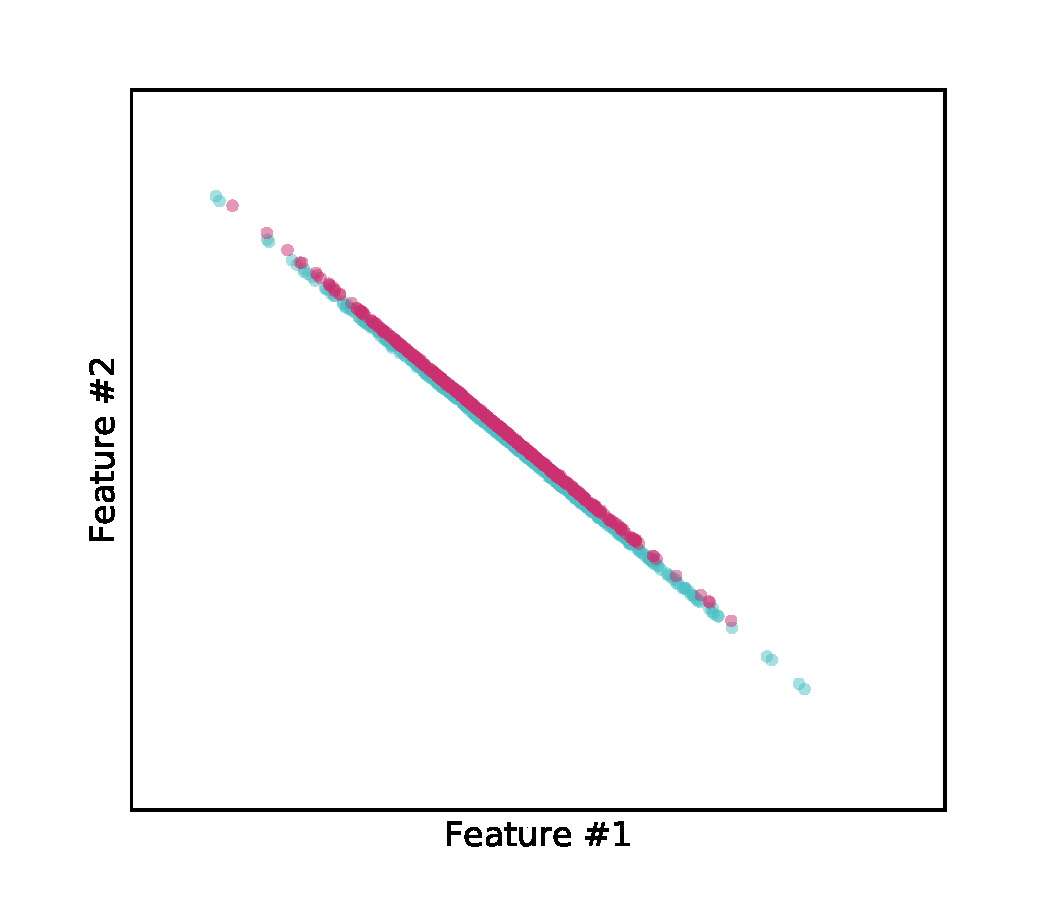
\includegraphics[width=.48\textwidth]{img/ML/ML_DL_original}\label{fig:ML:DL_original}} \hfil
	\subfloat[Visualization of the constraints used for the example]{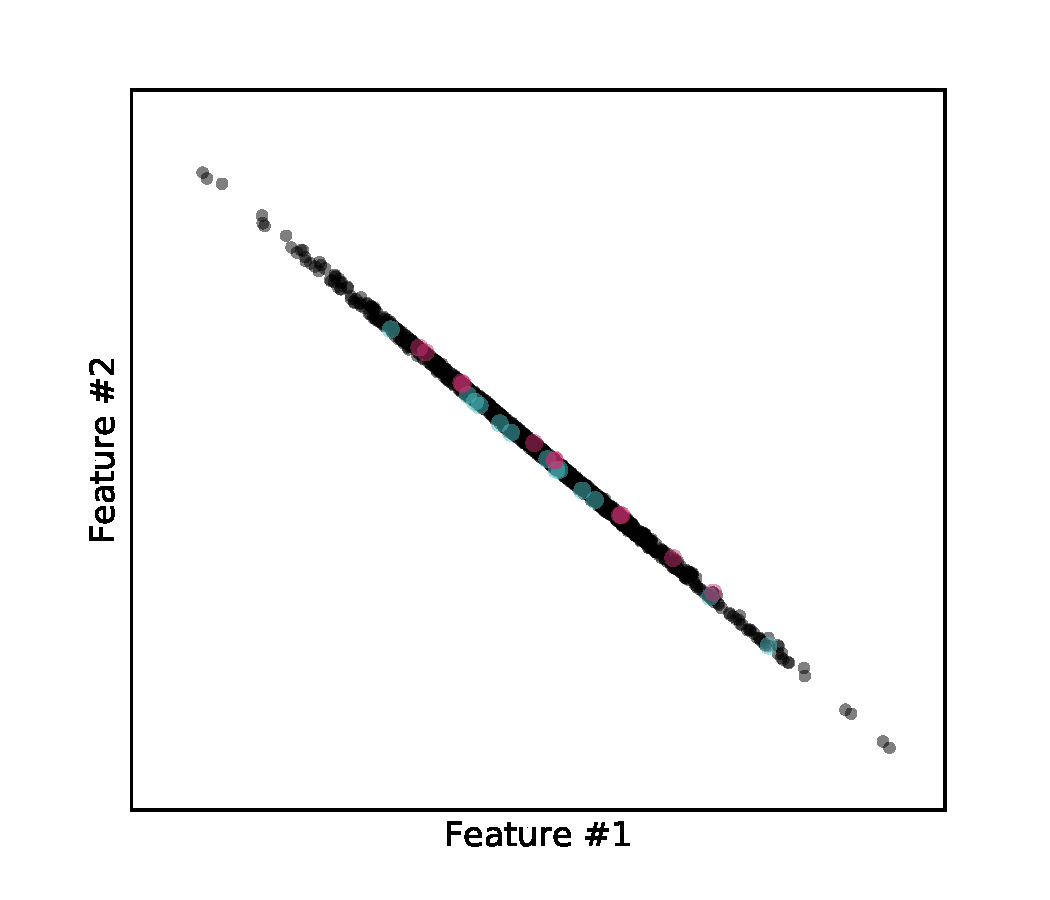
\includegraphics[width=.48\textwidth]{img/ML/ML_DL_constraints}\label{fig:ML:DL_constraints}}
	\caption{Generic distribution and constraints used for the example on distance learning}
	\label{fig:ML:DL_OC}         
\end{figure}

In Figure \ref{fig:ML:DL_OC} we present a visualization for an example of the distance learning techniques. Let us suppose to have data from two distributions, as shown in Figure \ref{fig:ML:DL_original}. We want to learn a distance metric able to assign high distances to samples in different distributions and low distances for samples in the same distributions. However, in our example scenario, we only rely on a few constraints shown in Figure \ref{fig:ML:DL_constraints}. Nevertheless, distance learning techniques are able to exploit the information provided by the constraints to learn a distance metric or a transformation of the space. In this work we use three techniques for distance learning. 

The first technique computes the Mahalanobis matrix by iteratively following some steps, and is therefore named \textit{Iterative Projection} \cite{xing2003distance} (IP). It defines a function $g(\mathbf{A})$ that estimates the sum of the Mahalanobis distances between the samples in the set $CL$ and a function $f(\mathbf{A})$ that estimates the sum of the Mahalanobis distances between the samples in the set $ML$. The goal is to maximize $g(\mathbf{A})$ and to minimize $f(\mathbf{A})$. The IP algorithm iteratively estimates the gradient of $g(\mathbf{A})$ with respect to $f(\mathbf{A})$ and makes use of a gradient ascent algorithm to converge to the optimal Mahalanobis matrix.

The second technique is named \textit{Relevant Components Analysis}\cite{bar2003learning} (RCA), because it performs an analysis of the relevance of each component for the computation of the distance. The RCA algorithm aims at assigning large weights to relevant dimensions and low weights to irrelevant ones. The relevance of the components are estimated within \textit{chunklets}, which are subsets of the data from the ML set. The Mahalanobis matrix is computed as the inverse of the covariance matrix of samples within the chunklets. This procedure reduces the relevance of the interaction of the components that exhibit a lower covariance.

The third technique is described in \cite{goldberger2004neighbourhood} and is named \textit{Neighborhood Components Analysis} (NCA), since it follows a nearest neighborhood approach. Such approach selects for each sample the $K$ nearest samples and define special properties for the samples that are mutual nearest neighborhood Specifically, the NCA algorithm aims at maximizing $f(\mathbf{A})$ the number of mutual nearest neighborhood samples among those defined in the $ML$ set. In order to do so, it applies a gradient ascent over $f(\mathbf{A})$ with respect to $\mathbf{A}$.

\begin{figure}[tb]
	\centering
	\subfloat[IP applied to the example ]{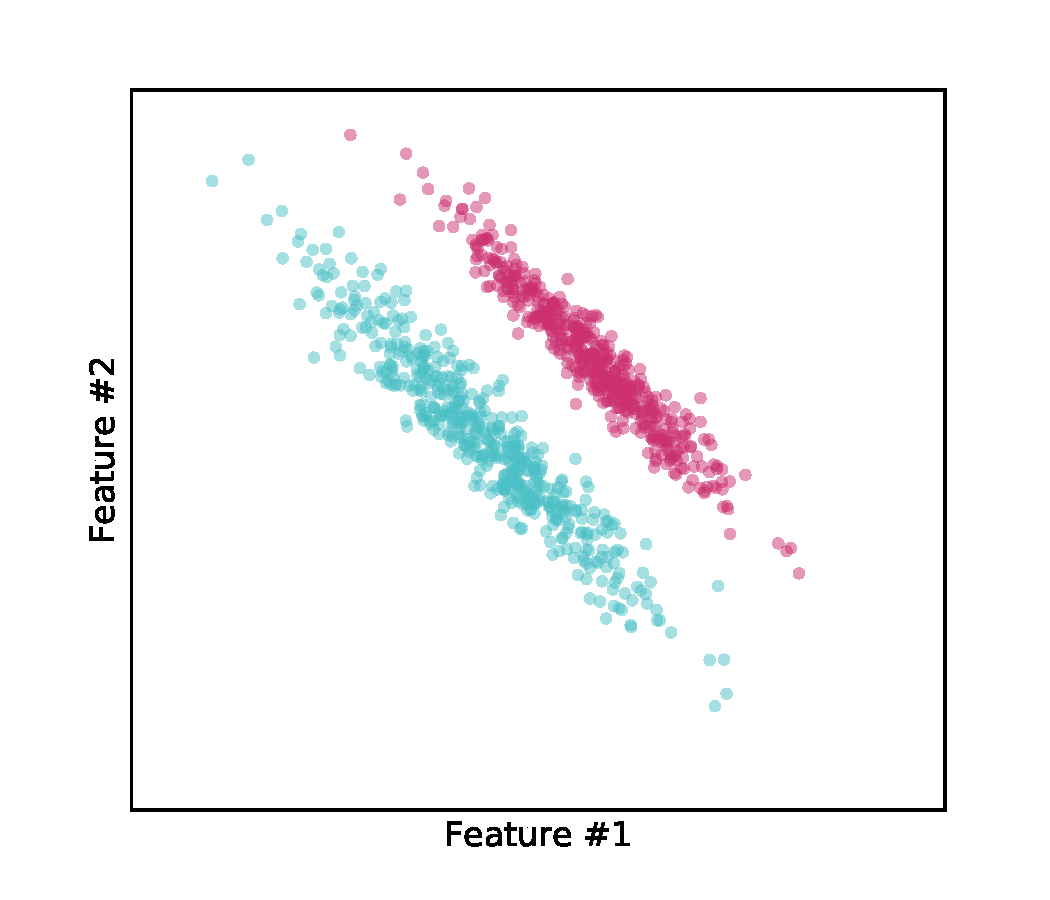
\includegraphics[width=.33\textwidth]{img/ML/ML_DL_IP}\label{fig:ML:DL_IP}} \hfil
	\subfloat[RCA applied to the example ]{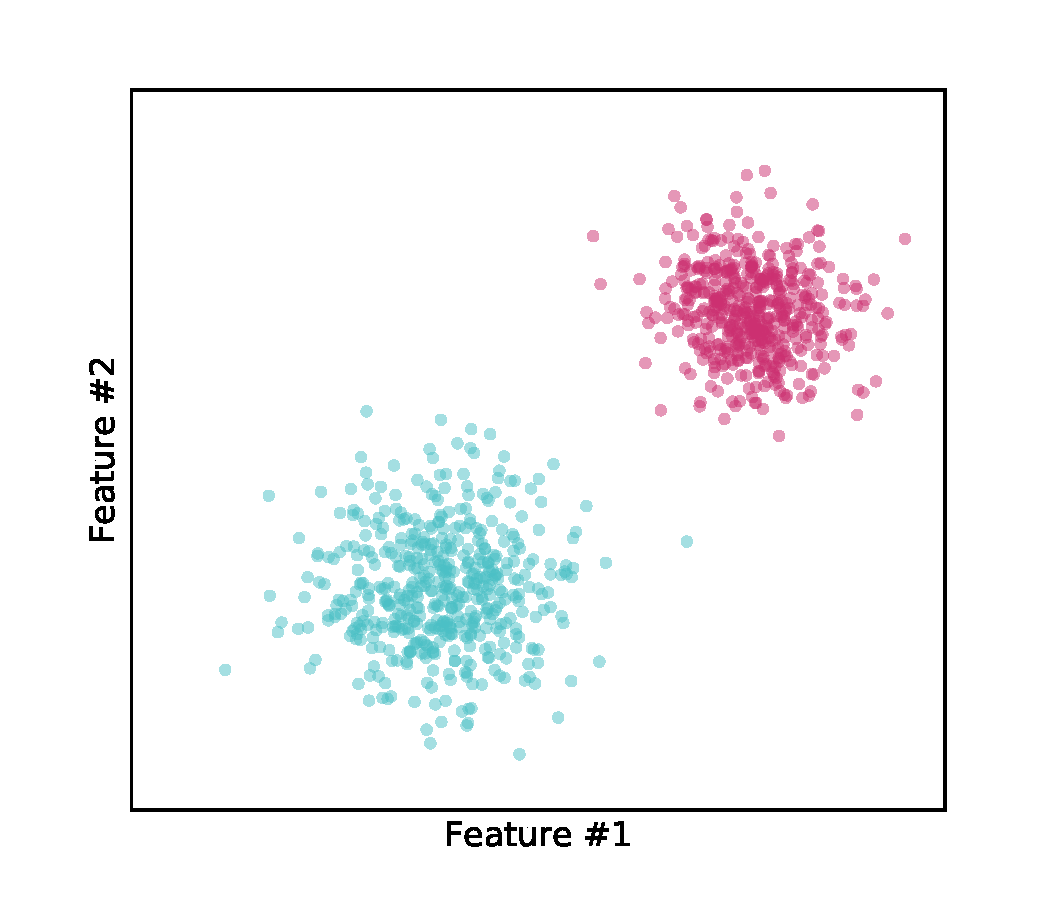
\includegraphics[width=.33\textwidth]{img/ML/ML_DL_RCA}\label{fig:ML:DL_RCA}} \hfil		
	\subfloat[NCA applied to the example ]{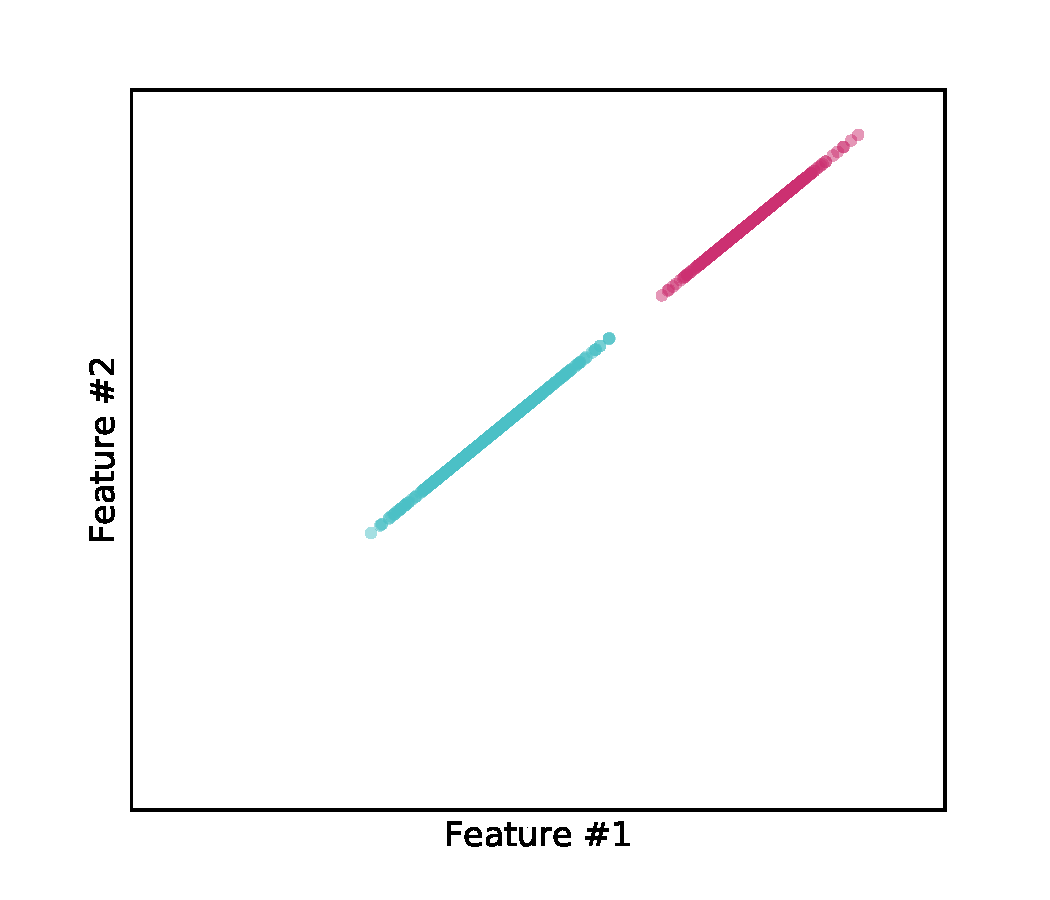
\includegraphics[width=.33\textwidth]{img/ML/ML_DL_NCA}\label{fig:ML:DL_NCA}} 
	\caption{Examples of the application of different distance learning techniques}
	\label{fig:ML:DL_IPNCARCA}         
\end{figure}

In Figure \ref{fig:ML:DL_IPNCARCA} we show the behavior of the three techniques for the example provided in Figure \ref{fig:ML:DL_OC}. We compute the transformation matrix $\mathbf{L}$ with the techniques and we apply them to the original distribution of data.  The IP algorithm shown in Fig. \ref{fig:ML:DL_IP}, is able to well separate the two distributions. However, we notice that the centroids of the distribution are closer with each other than with the samples at the edge of their distribution. The same drawback appears when NCA technique is applied (Fig. \ref{fig:ML:DL_NCA}), where the shape of the distribution is also somehow preserved. In this example, the best performance is provided by the RCA technique, in Fig. \ref{fig:ML:DL_RCA}, which manages to well separate the two distributions and also reduce the distance between samples in the same distribution. It is worth noting that we can not draw conclusions on the effectiveness of the techniques from this example alone. Nevertheless, we observe that all the techniques are able to detect and separate the two distributions from a set of few constraints.

\subsection{Machine Learning techniques for classification}\label{sec:ML:classifiers}
In the machine learning literature, a classifier is defined as a model that aims at predicting a categorical outcome from the input data \cite{PAMI}. The classifiers can be used whenever the codomain of the problem is formalized with discrete values. In this Section we provide a review for two main approaches for classification: the linear classifier and the Support Vector Machine (SVM).


%The music classification (Section \ref{sec:HLFs:class}) and categorical annotations (Section \ref{sec:HLFs:anns}) have in common the basic approach to formalize the semantic codomain, i.e., to predict whether a certain HLF can be used to describe a certain music piece. In the former scenario, a set of labels can be defined to fully define the semantic codomain. In the latter scenario a set of descriptors is defined, and each descriptor performs a partition of the codomain into the presence or absence of the related characteristics. Both problems can be addressed by modeling the linking function as a classifier. 

%If we aim at classifying a certain frame $\iota$ into $P$ non-overlapping labels, we can model the desired output as a matrix $\mathbf{Y} \in \{-1,+1\}^{F\times P}$ where each row $\mathbf{y}_\iota \in \mathbb{R}^{1 \times P}$ has a value equal to $+1$ in the $p$-th component relative to the label of the $\iota$-th sample and $-1$ otherwise. If we aim at annotating the frame within a set of $P$ descriptors instead, we set $\mathbf{y}_\iota^{(p)}=+1$ to indicate the presence of the $p$-th HLF in the description of the $\iota$-th frame, and $\mathbf{y}_\iota^{(p)}=$ to indicate its absence. 

The linear classifier is the most simple classifier, and it assumes that the outcome of a model can be predicted as a linear combination of the input components. Let us consider the simplest case, a two-class classifier where each outcome is formalized as $y_i=\{-1,+1\}$ depending on which class it belongs to. The linear classifier predicts the outcome as: 
\begin{equation}
\hat{\mathbf{Y}}=\tilde{\mathbf{X}} \mathbf{b},
\label{eq:ML:linClassPred}
\end{equation}
where $\tilde{\mathbf{X}}$ is the regularized representation of the domain, $\mathbf{b} \in \mathbb{R}^{M}$ is the vector of parameters for the classifier and $\hat{\mathbf{Y}}$ are the predicted values. 

The linear classifier is trained in order to learn the vector $\mathbf{b}$, i.e., the weights of the linear combination. More specifically, each component $\mathbf{b}_m$ represents the weighting for the $m$-th input component. The predicted output $\hat{\mathbf{Y}}$ is actually continuous and needs to be discretized by applying the sign function component-wise over the vector $\hat{\mathbf{Y}}$, in order to estimate the final class.

The learning of the parameters for the linear classifier is trivial, since it only involves the multiplication of the pseudo-inverse of the input matrix $\tilde{\mathbf{X}}$ with the expected outcome $\mathbf{Y}$ :
\begin{equation}
\mathbf{b}=(\tilde{\mathbf{X}}\T \tilde{\mathbf{X}})^{-1}  \tilde{\mathbf{X}}\T  \mathbf{Y}.
\label{eq:ML:linClass}
\end{equation}

The linear classifier can be generalized in the number of classes and in the number of total classifiers. If we need to estimate a set of $P$ 2-class classifiers for the input data, i.e., $ \mathbf{y}_i \in \{-1,+1\}^P$, we generalize the model by simply considering a matrix of
output data $\mathbf{Y}$  and predicted output data $\hat{\mathbf{Y}}$, both with $N$ rows (the number of samples, and $P$ columns (the number of classifiers). By substituting the matrix  $\mathbf{Y}$  in Equation \ref{eq:ML:linClass}, we obtain the matrix of parameters $\mathbf{B}\in\mathbb{R}^{M \times P}$, where each column $\mathbf{B}^{(p)}$ takes the role of the vector of parameters $\mathbf{b}$. The matrix is used in Equation \ref{eq:ML:linClassPred}, with the same discretization of $\hat{\mathbf{Y}}$ performed column-wise.

If, instead, we need to train a $P$-class classifiers, we still use a formalization of the output data such that $ \mathbf{y}_i=\{-1,+1\}^P$, where $ \mathbf{y}_i^{(p)}=+1$ if $x_i$ belongs to the $p$-th class and $ \mathbf{y}_i^{(p)}=-1$ otherwise. This approach is referred to as one-versus-all \cite{Manning2008}. The same Equations \ref{eq:ML:linClassPred} and \ref{eq:ML:linClassPred} hold also for this case, while the interpretation of the matrix of parameters $\mathbf{B}\in \mathbb{R}^{P \times M}$ is slightly different: each column $\mathbf{B}^{(p)}$, indeed, represents a model specifically trained for the $p$-th class, i.e., it is similar to train $P$ 2-class classifiers, each of them aims at predicting the $p$-th class. The discretization of $\hat{\mathbf{Y}}$ also changes. In this case, we assign each  sample to the class that is predicted with a higher likelihood. In order to do so, we consider each row $\hat{\mathbf{y}}_i$, and we compose a vector with all components equal to $-1$ except for $\hat{\mathbf{y}}_i^{(q)}=+1$ , with $q=\argmax{p} \hat{\mathbf{y}}_i^{(p)}$. 

The linear classifier has a simple geometric interpretation: each vector $\mathbf{b}$ defines a manifold in the input space that is  shaped in order to have high values where the input samples of a certain class are more likely to be distributed and low values where they are not. 

\begin{figure}[tbp]
	\begin{center}
		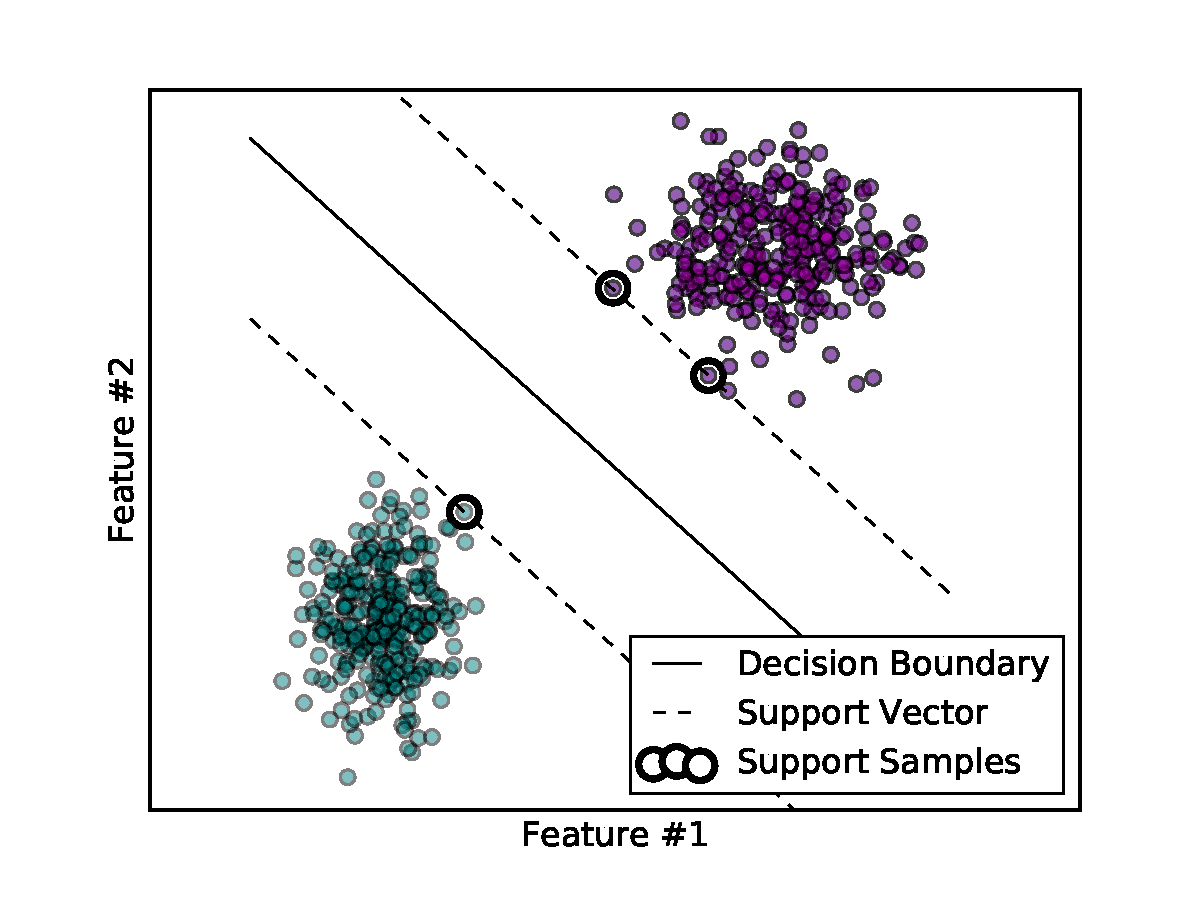
\includegraphics[width=12cm]{img/ML/ML_SVM}
		%\psfig{file=img/ML/logopm.jpg,width=3.5cm}
	\end{center}
	\caption{A graphic representation of the SVM classifier}
	\label{fig:ML:SVM}
\end{figure}

The Support Vector Machine (SVM) classifier follows a different approach, by learning the hyperplane that separates the input data that belong to a certain class from those that do not. The hyperplane is designed in order to have the maximum possible separation between the classes. In order to do so, the SVM technique relies on \textit{support vectors}, that are the vectors that connect the samples of the two classes which are closer to a given hyperplane, i.e., the \textit{support samples}. Maximizing the distance between the hyperplane and the support vectors leads to a better separation between classes. We show a representation of the behavior of SVM in Figure \ref{fig:ML:SVM}.

The SVM is a binary classifier, i.e., it only learns a hyperplane that separates two classes. However, we generalize its behavior using the aforementioned one-versus-all strategy by learning $P$ SVMs, each of which separates the samples that belong to the $p$-th class from those that do not. The final prediction is actually similar to the one for the linear classifier: the label that achieves the higher likelihood is assigned to the sample.

The SVM classification is a simple application of the hyperplane $\mathbf{w}\in \mathbb{R}^{M}$ to the generic frame $\mathbf{x}_i$ such that
\begin{equation}
\hat{y}_i=\text{sign}(\mathbf{w}\T \mathbf{x}_i + b)
\end{equation}
where $y_i$ indicates the predicted output for a generic SVM and $b$ is the intercept of the hyperplane. We learn the manifold by solving the minimization problem:
\begin{equation}
\begin{split}
\min  ||\mathbf{w}||^2\\
\text{subject to  } y_i(\mathbf{w}\T \mathbf{x}_i)\geq 1 \\
\forall i=1,...,N
\end{split}
\label{eq:ML:SVM}
\end{equation}

%The two class problem is usually generalized to multi-class problems by training several SVM classifiers, where each of them classify whether a sample belongs to a certain class and the class that has a higher estimated value is assigned to the sample.

Both the linear and SVM classifiers use a linear combination of the input to design the classification function. However, they can exploit nonlinearity relationship between features by using kernel expansion techniques presented in Section \ref{sec:ML:kernels}. This allows the two classifiers to learn decision surfaces that are nonlinear with respect to the feature space, empowering the predictive power of the models.

%The two classifiers are still linear with respect to the components, but since the components are now a nonlinear transformation of the original input space, it results in a decision function that is nonlinear in the input space.

In this thesis we use classification techniques in Chapter \ref{Chap:Bootleg}, to model a linking function from a representation of the signal domain to a non-overlapping labeling of the semantic domain.


\subsection{Machine Learning techniques for regression}\label{sec:ML:semantics}
Regressors are defined as machine learning techniques that are able to predict an outcome within a continuous range of values. In this section we provide an overview of the regressor techniques we use in our work. We use a similar notation as in Section \ref{sec:ML:classifiers}, with the expected normalized output defined as $\mathbf{Y}\in [0,1]^{N \times P}$.
%, where each column $\mathbb{Y}^{p}$ with $p=1,...,P$ models the $p$-th descriptor.

Similarly to the linear classifier (Section \ref{sec:ML:classifiers}), we can model a regressor as a linear combination of the input components \cite{Sen1990}. The linear regression \cite{PAMI} is based on the same principle of the linear classifier, hence we use the same Equations \ref{eq:ML:linClassPred}, \ref{eq:ML:linClass} to learn the parameters and compute the predicted values, by using the dimensional definition of $\mathbf{Y}$. From a geometric interpretation a linear regression model aims at learning the manifold that minimizes the squared distance between the manifold at a given point (i.e., the predicted value) and the correspondent expected value.

The linear approach is simple but often effective to model the linking function. However, it may also lead to overfitting, i.e., to learn a model that fits too much the training data and it is not general for the real-case scenario. The Ridge Regressor addresses the over-fitting issue by setting a constraint on the sums of the parameters of the linear combination \cite{PAMI}, i.e., on the maximum $||\mathbf{b}||$ in Equation \ref{eq:ML:linClass}. The constraint forces the model to share the predictive power of the weights of the linear combination, hence to focus on the more informative components. This leads to a higher training error, but it often achieves higher performance in the real world scenario. Given the parameter $\lambda$, related to the constraint on the sum of parameters, we train the parameters of the model by computing \cite{PAMI}
\begin{equation}
\mathbf{B}^{ridge}=(\mathbf{X}\T \mathbf{X}+\lambda \mathbf{I})^{-1}  \mathbf{X}\T  \mathbf{Y}.
\label{eq:ML:ridge}
\end{equation}
The constraint on the sum of parameters is a common regularization method also known as \textit{weight decay}.

\begin{figure}[tbp]
	\begin{center}
		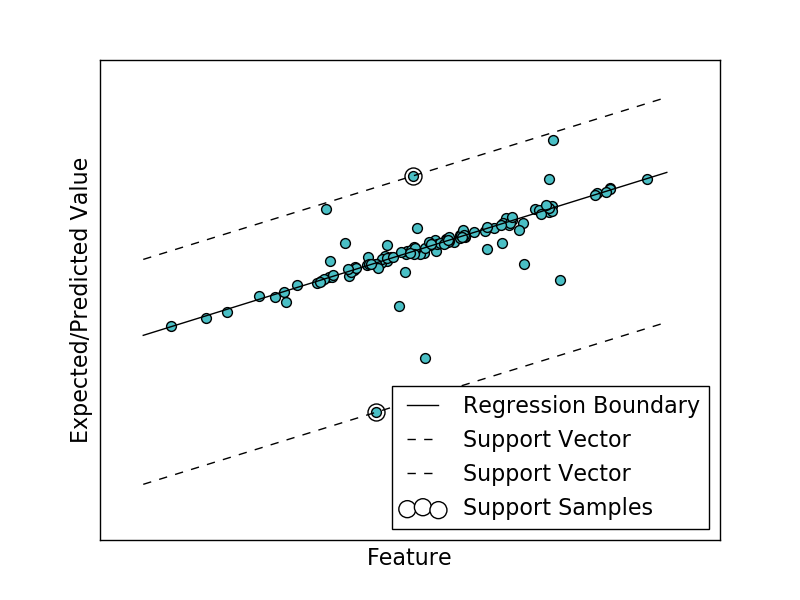
\includegraphics[width=12cm]{img/ML/ML_SVR}
		%\psfig{file=img/ML/logopm.jpg,width=3.5cm}
	\end{center}
	\caption{A graphic representation of the SVR regressor}
	\label{fig:ML:SVR}
\end{figure}

A similar parallelism between linear classifier and regressor also holds for the Support Vector Machine. The support vectors are used to predict a continuous value by using the Support Vector Regression (SVR) model \cite{Rho2009}. While in classification the support vectors are used to find the manifold that maximizes the separation between classes, in the regression problem the support vectors identify the manifold that minimizes the mean squared error of samples, as shown in Figure \ref{fig:ML:SVR}. With respect to the minimization problem of Equation \ref{eq:ML:SVM}, in the SVR we want to minimize
\begin{equation}
\begin{split}
\min  ||\mathbf{w}||^2\\
\text{subject to  } (y_i-\mathbf{w}\T \mathbf{x}_i)^2\leq \epsilon^2 \\
\forall i=1,...,N
\end{split}
\label{eq:ML:SVR}
\end{equation}
where $\epsilon$ is the maximum allowed error.

The linear and ridge regression models are based on the assumption that the output value can be predicted as a (possibly constrained) linear combination of the components. In order to overcome the limitations of the linearity assumption, we exploit the kernel expansion discussed in Section \ref{sec:ML:kernels}.

As an example, we use the polynomial kernel to expand the data and include nonlinearity in the computation. Performing a linear regression on polynomial-expanded data is referred to as polynomial regression \cite{Sen1990}. The prediction model of the polynomial regression is linear with respect to the expanded data, which means it is nonlinear with respect to the original data. It is also common to use the Radial Basis Function kernel for the SVR model, in order to benefit the design of the manifold with nonlinear shapes \cite{Smola2004}. 

The mentioned techniques estimate the parameters of their model by minimizing the training error, i.e., the prediction error over the samples in the training set. The training error can also be used to guide the learning process. In boosting methods, the prediction model is composed by several estimators, each taking care of a subset of the training set where the error is higher. This allows the estimators to focus on the samples that are more difficult to model, and therefore to provide a better prediction model. In this work we use two boosting methods, which are the AdaBoost and Gradient Boost regressors. 

The AdaBoost regressor \cite{Solomatine2004} follows the boosting approach by assigning a weight to each sample of the training set. The values of the weights define which samples should be seen as more important for the training step. At first, the weights are equal for each sample, so the regressor learns the same model for each sample. After one iteration, the training error is estimated for each sample and the weights are adapted such that the samples with higher error receive higher weights and vice versa. The model is trained again with the updated weights, and a new prediction error is estimated, which leads to the definition of new weights. The process is iterated several times and leads to the learning of a general model that is able to deal with both trivial and complex samples.

The Gradient Boost regressor \cite{Zemel2001} uses a similar approach of AdaBoost, while collecting the estimator models through the iterations. The first iteration of the algorithm works as in the AdaBoost model. In the second iteration, however, the outcome is estimated as a linear combination of the models learned in the first and in the second iteration. The weights of the combination $c_1$ and $c_2$ are chosen through a linear search to minimize the total training error. The weights for the samples are then updated using a gradient descent approach that makes use of the weight of the last retrieved model. After a set of $T$ iterations, the final prediction model is composed by the linear combination of the $T$ models retrieved at each iteration. The lower the training error of a model at a given iteration, the higher its weight, and therefore its relevance, in the final combination of models.

All the machine learning algorithms we just described for regression problems are able to model a linking function between a representation of the domain and a dimensional codomain. In Section \ref{sec:LLFs:learned} we described how deep neural networks are employed to automatically extract a feature representation of the signal domain. Neural networks are also employed to model the linking function, as example, by means of an architecture named \textit{Multilayer Perceptron} (MLP) \cite{PAMI}. 

A MLP is a machine learning architecture which is composed of a hidden layer, represented by a denoising autoencoder (Section \ref{sec:LLFs:learned}), and an output layer that predicts its outcome from the extracted features in the hidden layer. The hidden layer extracts a representation of the input so that the input can be reconstructed from it, while the output layer learns the linking function to the desired predicted value \cite{PAMI}. The MLP cannot be considered a deep learning technique, since it is composed by only two layers, as shown in Figure \ref{fig:ML:MLP}, and therefore it shows moderate performance in the prediction. Nevertheless, its swallow architecture makes it a computationally affordable solution to learn some kind of automatic representation from the domain and link it directly to the codomain. The MLP is typically trained in two steps:
\begin{enumerate}
	\item
	a \textit{forward stage}, in which the hidden layer $h$ and output $O$ are computed;
	\item
	a \textit{backward stage}, in which the prediction error is computed and then used for correcting the parameters of the hidden and output layer
\end{enumerate}
Forward and backward steps are repeated for a certain amount of iterations, before approaching the global minimum error, in order to avoid overfitting issues \cite{PAMI}.

\begin{figure}[tbp]
	\centering
	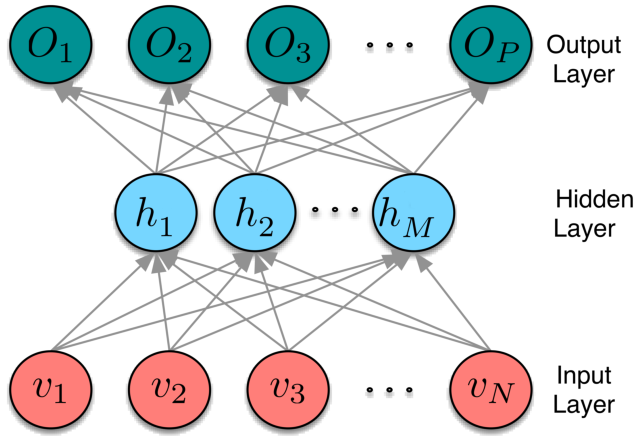
\includegraphics[width=.6\textwidth]{img/ML/MLP.pdf}
	\caption{General representation of a MLP}
	\label{fig:ML:MLP}
\end{figure} 

\section{Final considerations}
The design and development of the linking function need to take into considerations the domain and codomain of the addressed problems. The former needs to be shaped for the linking function, involving the regularization of the representation, and a possible expansion of the input space by means of kernel techniques. The linking function can be manually designed by means of rule-based techniques or learned by means of machine learning algorithms. We provided a background of rule-based techniques for the task of music structure analysis, which also involves the computation of the self-similarity and self-distance matrices as a useful representation of the music structure. We finally presented: a set of machine learning techniques for clustering, which involves unsupervised and semi-supervised techniques; distance learning techniques, in order to learn a semi-supervised distance metric for the input space; and completely supervised machine learning techniques to address codomain represented by discrete (classifiers) or continuous range (regressors).

%In the following chapters, we discuss a set of scenarios to model the music perception with increasing complexity. We employ the techniques described in Chapters \ref{Chap:LLFs}, \ref{Chap:HLFs} and \ref{Chap:ML}, to formalize the signal domain, the semantic codomain and to design a feasible and effective linking function.